\FloatBarrier\section{MPC} \label{sec:mpc}

    \paragraph
    \acrfull{MPC} refers to a control approach that determines the control action at each time-step 
    by solving an open-loop optimal control problem over a finite prediction horizon \cite{Mayne2000}.
    \gls{MPC} does not refer to a specific algorithm implementation, but rather to the general control approach.

    \begin{figure}[ht]
        \centering
        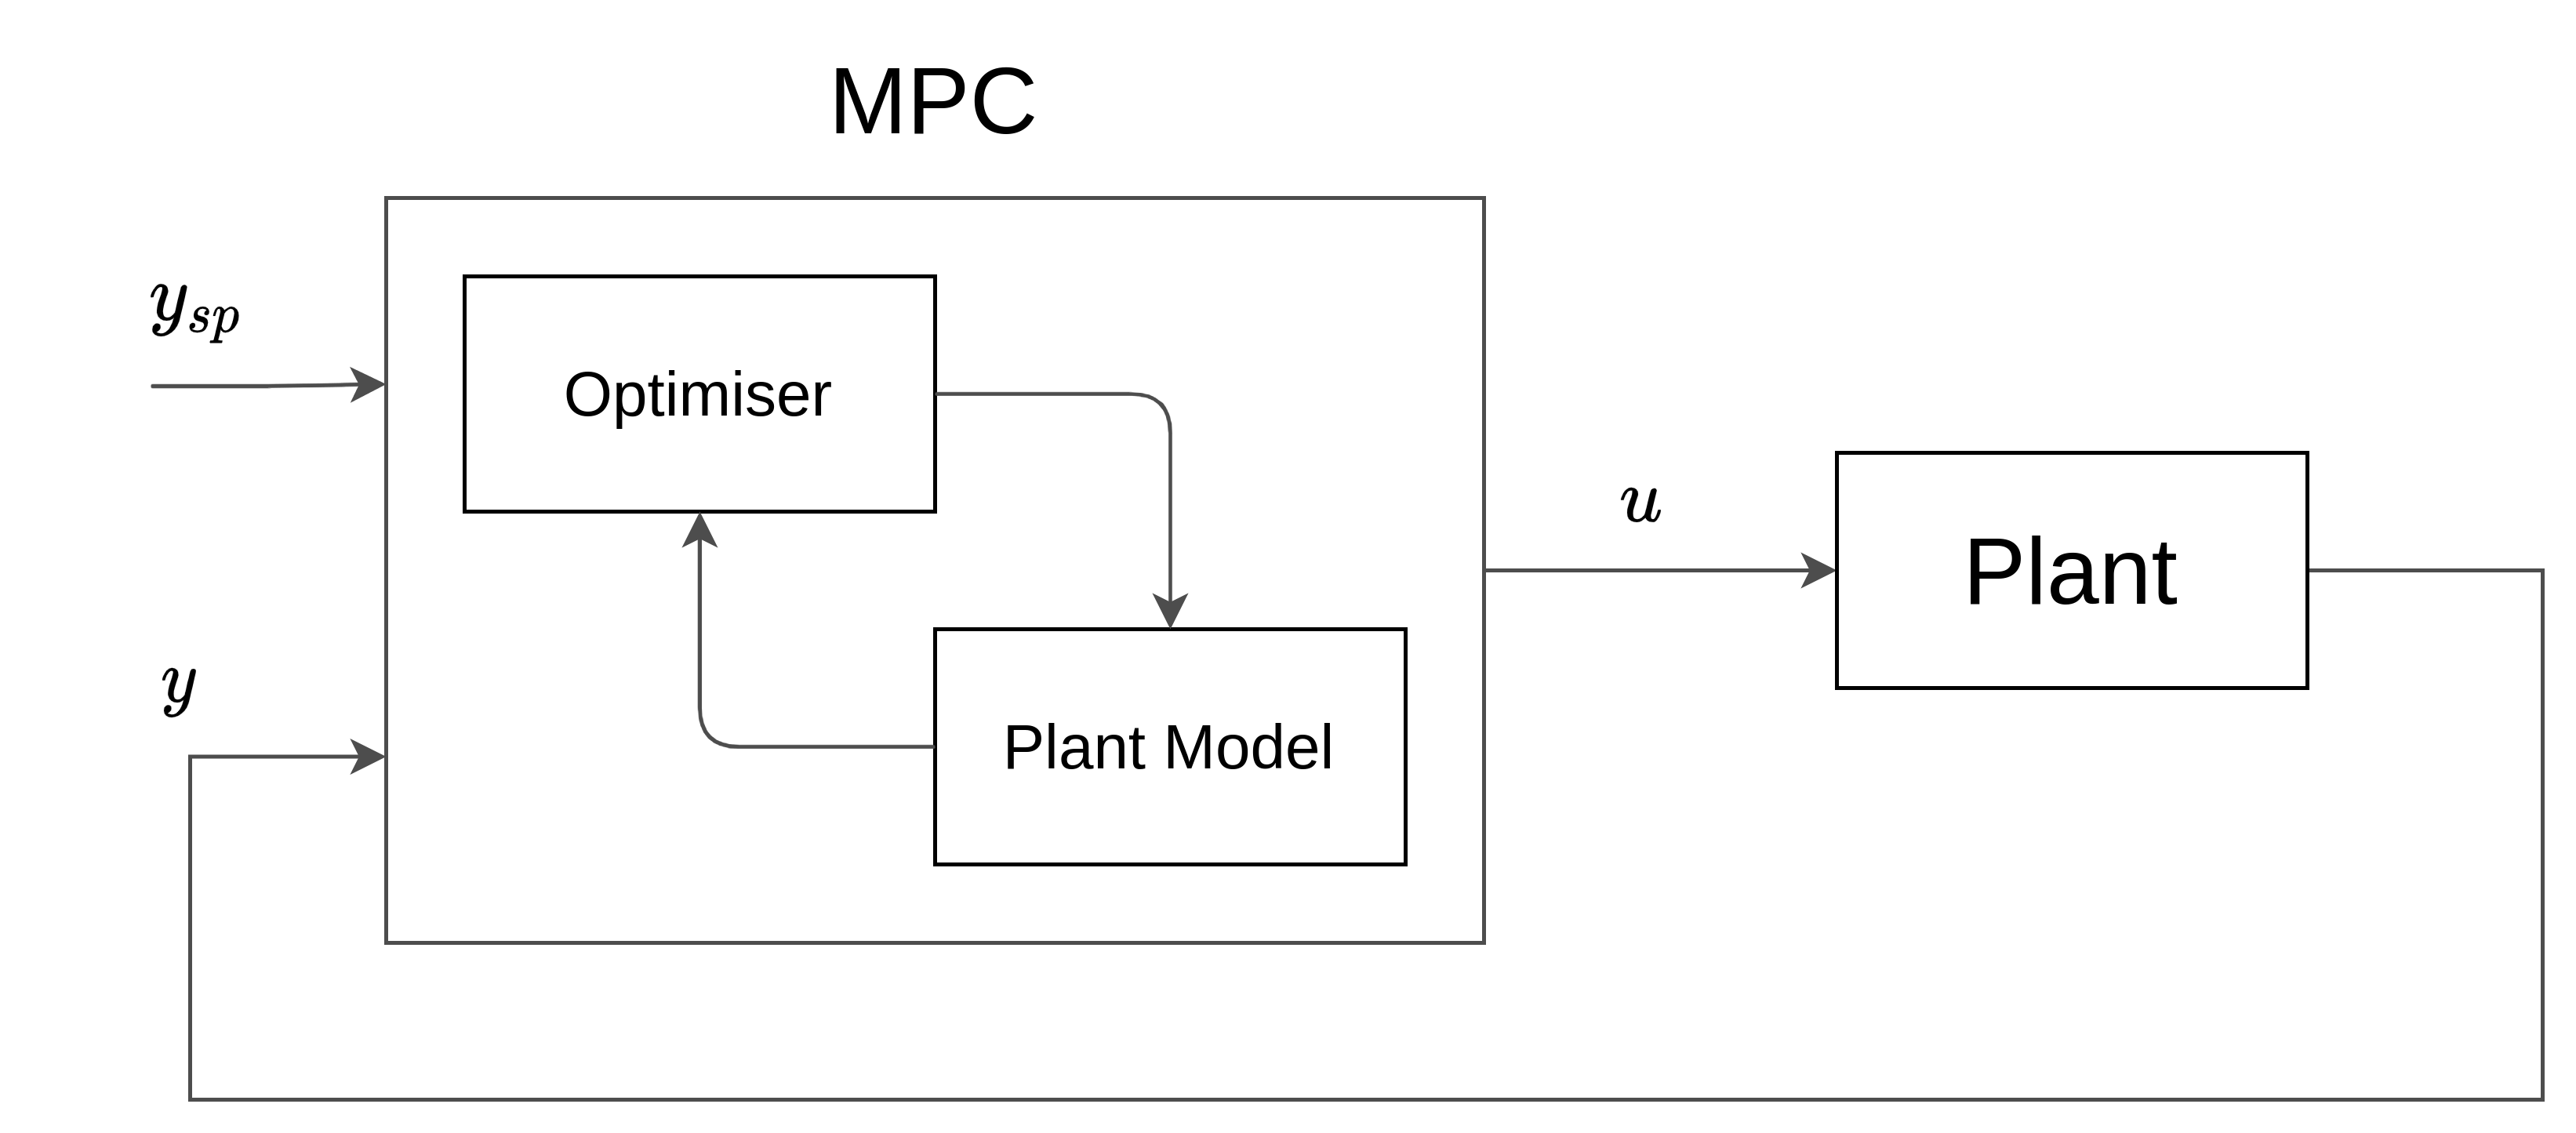
\includegraphics[width=0.818\linewidth]{control/fig/MPC_controller}
        \caption{Diagram of the structure of a typical MPC}
        \label{fig:mpc_controller}
    \end{figure}
% ?? remove all MV and MO
    \paragraph
    Shows the structure of a typical MPC implemnetation.
    As a high-level overview, the MPC receives the measured output vector, $\bm{y}$, 
    and the output setpoint $\bm{y}_{sp}$, and detemines the control action, $\bm{u}$, to drive the $\bm{y}$ values to $\bm{y}_{sp}$.
    An optimiser uses an internal plant model to determine an optimal control sequence over a prediction horizon \cite{Mayne2000}.
    Therefore $\bm{y}_{sp}$ may be replaced by a target trajectory for the prediction horizon. 
    Only the first control action of the optimal sequence is expecuted and the optimisation is re-calculated at every time-step.

    \paragraph
    Each specific \gls{MPC} implementation is dependant on the plant model representation \cite{Garcia1989}.
    In this section, an overview will be given of the specific \gls{MPC} implementation used in this work.
    Similarly to the presented \gls{PID} and \gls{LQR} controllers, the presented \gls{MPC} 
    The \gls{MPC} objective function will be explained and the design process to tune the controller will be discussed.
    It will also be discussed how integral action is achieved with the \gls{MPC}.
    Finally, the control response of the tuned \gls{MPC} will be shown and discussed for a simulated system.

    \FloatBarrier\subsection{Plant model} \label{sec:mpc_model}

        \paragraph
        An estimated model from the data-driven techniques discussed in Chapter~\ref{chap:system_id} will be used as the plant model 
        for the proposed \gls{MPC} architecture.
        \gls{DMDc} produces a discrete, linear state-space model of the system dynamics.
        Hence, an \gls{MPC} implementation that corresponds to such a model will be used.
        The following state-space model representation will be used,
        \begin{equation} \label{eq:mpc_state_space}
            \bm{x}_{mpc} (k+1) = \bm{A}_{mpc} \bm{x}_{mpc} (k) + \bm{B}_{mpc} \bm{u}_{mpc} (k) ,
        \end{equation}
        where
        $\bm{A}_{mpc}$ is the system matrix and
        $\bm{B}_{mpc}$ is the input matrix
        applied by the \gls{MPC}.
        $\bm{x}_{mpc} (k)$ is the state vector and
        $\bm{u}_{mpc} (k)$ is the input vector at time-step $k$
        for this state space model.
        It is assumed that full-state feedback is available.

        \paragraph
        \gls{DMDc} applies multiple delay-coordinates to account for input delay and state delay in the system.
        In Section~\ref{sec:dmdc}, it was shown that the \gls{DMDc} implementation produces three matrices, 
        $\bm{A}_{dmd}$, 
        $\bm{A}_d$, and 
        $\bm{B}_{dmd}$.
        However, the \gls{MPC} requires a single system matrix, $\bm{A}_{mpc}$. 
        Therefore the \gls{DMDc} system is converted into:
        \begin{align}
            % 
            \begin{bmatrix}
                \bm{x}_{dmd} (k+1) \\ \bm{d} (k+1)
            \end{bmatrix}
            &=
            \begin{bmatrix}
                \bm{A}_{dmd} & \bm{0} \\
                \bm{I}_d & \bm{0}
            \end{bmatrix}
            \begin{bmatrix}
                \bm{x}_{dmd} (k) \\ \bm{d} (k)
            \end{bmatrix}
            +
            \begin{bmatrix}
                \bm{B}_{dmd} \\ \bm{0}
            \end{bmatrix}
            \bm{u}_{dmd} (k) ,
            \\ 
            \phantom{\begin{bmatrix} . \\ . \end{bmatrix}} % To get vertical spacing right
            \bm{x}_{mpc} (k+1) \hspace{7pt}
            &=
            \hspace{15pt} \bm{A}_{mpc} 
            \hspace{25pt} \bm{x}_{mpc} (k) 
            \hspace{7pt} + 
            \hspace{7pt} \bm{B}_{mpc} 
            \hspace{9pt} \bm{u}_{mpc} (k) ,
            % 
        \end{align}
        where $\bm{I}_d$ is the indentity matrix that links the corresponding entries in $[ \bm{x}_{dmd} (k) ~~ \bm{d} (k) ]^T$ to $\bm{d}(k+1)$.
        This produces large state-space matrices with many unneccesary output variables in $\bm{d}(k+1)$.
        To ignore these variables in the control optimisation, they are all assigned a zero weight in the \gls{MPC} objective function.
        The objective function will be discussed in the sections below.

        % ?? correct \gls
        % ?? State space model with $A_{mpc}$

        \paragraph
        Recall from Section~\ref{sec:payload_state_variable} that $\dot{\theta}$ is not used in the estimated model.
        However, as discussed in Section~\ref{sec:lqr}, it is better for a controller to minimise $\dot{\theta}$, 
        rather than $\theta$, because $\theta$ has a non-zero steady-state value due to aerodynamic drag during a veloicty step response.
        The state vector is therefore augmented with the $\dot{\theta}$ variable, such that the state vector is rather given by,
        \begin{equation}
            {\bm{x}_{mpc}}^T = 
                \begin{bmatrix}
                    V_N & \theta & \dot{\theta} & \bm{d}
                \end{bmatrix} , \phantom{~~~}
        \end{equation}
        where $\bm{d}$ is the delay state vector defined in Equation~\ref{eq:delay_vector}.
        The $\bm{A}_{mpc}$ matrix is also augmented with the Backwards Euler numerical differentiation equation, such that,
        \begin{equation}
            \dot{\theta} (k) = \frac{1}{T_s} \theta(k) - \frac{1}{T_s} \theta(k-1) 
        \end{equation}
        $\bm{B}_{mpc}$ is also changed such that the matrix dimentions agree but $\bm{u}_{mpc} (k)$ does not directly influence $\dot{\theta} (k)$.
        In this way, a weight can be applied to the $\dot{\theta}$ variable in the \gls{MPC} objective function to control this variable.

    \FloatBarrier\subsection{Receding horizon}

        \paragraph
        Diagram of prediction horizon and control horizon

        % ?? See \cite{Mayne2000} for good intro to

        \paragraph
        controller desicion, ${z_k}^T = [ u( k | k )^T ~~ u( k+1 | k)^T ~~ ... ~~ u( k+p-1 | k )^T ] $

    \FloatBarrier\subsection{Algoriithm}

        \paragraph
        Different implementations. e.g. list
        Based on model
        Other \gls{MPC} optimiser options.
        MATLAB chosen. Why MATLAB?
        C++ generation
        
        \paragraph
        The \gls{MPC} implementation from the Model Predictive Control Toolbox\texttrademark ~solves the control optimisattion problem as a \gls{QP} at each time interval \cite{MPCtoolbox2019}.
        This QP usually consists of three features, namely,
        \begin{itemize}
            \item the objective function,
            \item the constraints, and
            \item the controller desion
        \end{itemize}
        The objective function provides a scalar value that quatifies the controller performance.
        The controller desicion is the $\bm{u}_{mpc}$ adjustments determined by the QP solver that minimise the objective function.
        The constraints are conditions that the controller decision need to satisfy, such as bounds on $\bm{x}_{mpc}$, $\bm{u}_{mpc}$, and $\Delta\bm{u}_{mpc}$ values.

        \paragraph
        Constraints cause non-linear ..., 
        not applied

        \paragraph
        The objective function used by the Model Predictive Control Toolbox\texttrademark is documented well by the corresponding user manual \cite{MPCtoolbox2019}.
        An overview of this implementation, which is used in this work, will be given here. 
        The objective function consists of the sum of three terms that each quantify a specific aspect of the control performance,
        and is calculated as,
        \begin{equation}
            J(z_k) = J_y(z_k) + J_u(z_k) + J_{\Delta u}(z_k),
        \end{equation}
        where $z_k$ is the controller decison at time-step $k$.
        The three scalar performance measures are denoted as
        $J_y(z_k)$ for output setpoint tracking,
        $J_u(z_k)$ for \gls{MV} tracking, and
        $J_{\delta u}(z_k)$ for \gls{MV} move suppression
        Each performance measure includes weigths that balanse the competing objectives of the different terms.
        These weights need to be manually tuned for a desired controller performance.

        \paragraph
        \textbf{Output setpoint tracking}  \newline
        The performance measure of the output setpoint tracking is calulated as,
        \begin{equation}
            J_y(z_k) = \sum_{j = 1}^{n_y} ~ \sum_{i = 1}^{N_p} 
                \left\{ 
                    {w^y}_{j} 
                        \left[ 
                            r_j( k+i | k) - y_j( k+i | k)
                        \right]
                \right\}^2 ,
        \end{equation}
        where the symbols are denoted as, \newline
        \begin{tabular}{ l l } 
            $k$             & Current control interval time-step. \\
            $n_y$           & Number of output variables. \\ 
            $N_p$           & Prediction horizon. \\ 
            $y_j( k+i | k)$ & Predicted value of $j$\textsuperscript{th} output variable at $i$\textsuperscript{th} time-step from $k$. \\
            $r_j( k+i | k)$ & Reference value of $j$\textsuperscript{th} output variable at $i$\textsuperscript{th} time-step from $k$. \\
            ${w^y}_{j}$     & Tuning weight for $j$\textsuperscript{th} output variable. \\
        \end{tabular}

        \paragraph
        The controller receives the reference values, $r_j( k+i | k)$, for the prediction horizon starting at time-step $k$.
        Using the inernal plant model, the predicted output values, $y_j( k+i | k)$, is determined based on the controller decision, $z_k$.
        The values of $N_p$ and ${w^y}_{j}$ are design choises and are constant controller specifications.
        The value of $n_y$ is also constant and is determined from the plant model.

        \paragraph
        \textbf{Manipulated variable tracking}  \newline
        In some control applications, it is desirable to keep specific \gls{MV} variables close to a target value.
        In the multirotor use case, lower \gls{MV} values are prefered because this corresponds to lower energy use.
        The \gls{MV} target values are therefore set to zero for our use case. 
        The performance measure of the manipulated variable tracking is calculated as,
        \begin{equation}
            J_u(z_k) = \sum_{j = 1}^{n_u} ~ \sum_{i = 0}^{N_p - 1} 
                \left\{ 
                    {w^u}_{j} 
                        \left[ 
                            u_j( k+i | k) - u_{j,sp}( k+i | k)
                        \right]
                \right\}^2 ,
        \end{equation}
        where the symbols are denoted as, \newline
        \begin{tabular}{ l l } 
            $n_u$           & Number of manipulated variables. \\ 
            $u_j( k+i | k)$ & Control decision of $j$\textsuperscript{th} \gls{MV} at $i$\textsuperscript{th} time-step from $k$. \\
            $u_{j,target}( k+i | k)$ & Target value of $j$\textsuperscript{th} \gls{MV} at $i$\textsuperscript{th} time-step from $k$. \\
            ${w^u}_{j}$   & Tuning weight for $j$\textsuperscript{th} \gls{MV}. \\
        \end{tabular}

        \paragraph
        The desired $u_{j,target}( k+i | k)$ values can be received for the prediction horizon starting at time-step $k$.
        However, for our use case, all $u_{j,target}( k+i | k)$ values are constant and zero.
        The value of $n_u$ is fixed by the plant model.
        The ${w^u}_{j}$ values are also constant and are determined as a design choise.
        
        \paragraph
        \textbf{Manipulated variable increment suppression}  \newline
        Large increments or moves in the \gls{MV} values is often undesirable for good control performance.
        In the multirotor use case, large increments of the acceleration \gls{MV}s result in large jerks which may cause the system to go beyond the accurate vector subspace of the plant model.
        High frequency moves in the acceleration \gls{MV}s may also cause jittery flight dynamics because acceleration setpoint changes correspond to attidue changes.
        The performance measure of \gls{MV} tracking is used to penalise increments in the \gls{MV}s.
        This is calulated as,
        \begin{equation}
            J_\Delta u (z_k) = \sum_{j = 1}^{n_u} ~ \sum_{i = 0}^{N_p - 1} 
                \left\{ 
                    {w^{\Delta u}}_{j} 
                        \left[ 
                            u_j( k+i | k) - u_j( k+i-1 | k)
                        \right]
                \right\}^2 ,
        \end{equation}
        where the symbols are denoted as, \newline
        \begin{tabular}{ l l } 
            ${w^u}_{j}$   & Tuning weight for movement in the $j$\textsuperscript{th} \gls{MV}. \\
        \end{tabular}

        \paragraph
        The values of ${w^{\Delta u}}_{j}$ are constant and are determined as a design choise.

        \paragraph
        The similarities and differences between the \gls{LQR} and \gls{MPC} objective functions should be noted.
        The \gls{LQR} implementation described in Section~\ref{sec:lqr}, did not included penalisation for MV increments.
        However, if $J_\Delta u (z_k)$ is removed from the objective function, the \gls{MPC} and \gls{LQR} controllers optimise the same variables.
        In both implementations weights are designed for these variables in the objective function.

        \paragraph
        The \gls{LQR} optimisation corresponds to solving the unconstrained \gls{MPC} optimisation problem for $N_p = \infty$.
        However, the \gls{LQR} optimisation is run only once to determine the \gls{LQR} gain, whereas the \gls{MPC} optimisation is re-run at every time-step.
        Also note that the \gls{LQR} uses a continuous-time model, but the \gls{MPC} considered in this work uses a discrete-time model.

% ?? convert acronyms to \gls{}

    \FloatBarrier\subsection{Integral action}
        
        \paragraph
        A simple implementation of predictive control with multiple output variables does not inherantly apply integral action or disturbance rejection.
        For the multirotor and suspeneded payload use case,
        \gls{MPC} control without integral action results in a non-zero steady-state error of the mulrtirotor velocity, due to wind distrubance and inaccuracies in modelling the drag.
        % Due to modelling inaccuraciose or disturbances, 
        % the \gls{MPC} may continually determine and execute a control action that does not drive the the If the actual aerodynamics drag is more than the drag accounted for in the model.
        % In this case, zero steady-state error tracking for every output variable will not be achieved in the presence of any model inaccuracy or disturbance.
        
        % A example can be used to explain this with the multirotor system.
        % Consider the case when the multirotor is flying at steady-state velocity and the payload angle is at steady-state.
        % The \gls{MPC} controls both the multirotor velocity and the payload angle.
        % A new velocity setpoint is given that is slightly large than the current velocity.
        % The \gls{MPC} optimiser will genertae a solution, $z_k$, to accelerate slowly to the new velocity setpoint without disturbing the paylaod angle too much. 
        
        \paragraph
        Different methods have been proposed to apply integral action with an \gls{MPC}.
        A commonly used method involves applying an integrator to the control action determined by the \gls{MPC} \cite{Ruscio2013}.
        In this implementation, the \gls{MPC} detemines the optimal control action increment, ${\Delta u_k}^*$,
        and the control action, $u_k = u_{k-1} + {\Delta u_k}^*$ is applied.
        Hence, ingtegral action is applied to the plant input.
        This method is also discribed by \cite{Mayne2000}.

        \paragraph
        Another commonly used strategy involves estimating a input disturbance in the plant model which influences an output variable \cite{Ruscio2013}.
        In this way, integral action is applied to the plant output.
        This is the integral action strategy applied in this work.
        Since integral action is required for $V_N$ in the North velocity controller,
        a disturbance model that influences $V_N$ is augmentented to the input matrix.
        
        \paragraph
        The resulting state-space matrix is,
        \begin{equation} \label{eq:mpc_ud_state_space_model}
            \bm{x}_{mpc} (k+1) = 
                \bm{A}_{mpc} \bm{x}_{mpc} (k) 
                + 
                \begin{bmatrix}
                    \bm{B}_{mpc} & \bm{B_{ud}}
                \end{bmatrix}
                \begin{bmatrix}
                    \bm{u}_{mpc} (k) \\ \hat{u}_{ud}(k)
                \end{bmatrix} ,
        \end{equation}
        where
        $\bm{B_{ud}}$ is the input disturbance model and 
        $\hat{u}_{ud}$ is the estimated input disturbance value.
        The input disturbance model is designed as,
        \begin{equation}
            \bm{B_{ud}} = 
                \begin{bmatrix}
                    0.1 & 0 & 0 & \bm{0}
                \end{bmatrix}^T ,
        \end{equation}
        such that it only influences $V_N$ in the state vector,
        \begin{equation}
            {\bm{x}_{mpc}}^T = 
                \begin{bmatrix}
                    V_N & \theta & \dot{\theta} & \bm{d}
                \end{bmatrix} . \phantom{~~~}
        \end{equation}
        
% ?? Talk about design of value 0.1 in distrubance model

        \paragraph
        The specific value of the non-zero matrix entry in $\bm{B_{ud}}$ has only a slight effect on the control performance, hence the interative tuning process for this value was simple.
        The value of $\hat{u}_{ud}(k)$ is estimated by the default Kalman filter estimator implemented by the Model Predictive Control Toolbox\texttrademark~ 
        using the state-space model from Equation~\ref{eq:mpc_ud_state_space_model}.
        The value of $\hat{u}_{ud}(k)$ is then used in the \gls{QP} solver to determine the optimal control action of the \gls{MPC}.
        The control performance was tested with the default Kalman filter gain with different payload parameters and disturbances.
        It was determined that the \gls{MPC} with the default input disturbance estimator provides acceptable controller performance without aditional tuning. 
        Hence, the default Kalman filter is used in the final control implementation.
        Zero steady-state error for velocity tracking was achieved for different paylaods and different input disturbacnes, showing that integral action is achieved.
        The simulation results showing the \gls{MPC} integral action will be shown and discussed in Section~\ref{sec:control_implementation}.

        % ?? plot showing difference between with integral action and without

    \FloatBarrier\subsection{Tuning}

        \paragraph
        In the controller tuning process, a large value of ${w^y}_{j}$ will correspond to more agrresive maneuvers of the $j$\textsuperscript{th} output variable, because of the tracking error of that variable will be heavily penalised.
        For the tuning process, small values of ${w^u}_{j}$, correspond to aggresive maneuvers, because the values of the \gls{MV}s are not heavily penalised in the objective function. 

        \paragraph
        The value of $N_p$ determines the number of decision values in $z_k$.
        Therefore the computational complexity of the QP problem increases with larger values of $N_p$.
        However, if the 
        Hence, the value of $N_p$ needs
        It is often state as a 

    \begin{figure}[htb]
    \centering
    \begin{tikzpicture}
        \begin{axis}[            
            xlabel = Time,
            ylabel = North velocity,
            x unit = \si{\second},
            y unit = \si{\metre/\second},
            xmin = 0,   xmax = 16,
            ymin = -0.1,  ymax = 2.4,
            grid = major,
            legend cell align = left,
            legend pos = south east,
            grid style = dashed,
            legend style = {font = \scriptsize},
            label style = {font = \scriptsize},
            tick label style = {font = \scriptsize},
            width = 0.95\columnwidth,
            height = 0.5\columnwidth,
            % initialize Dark2
            cycle list/Dark2,
            % combine it with 'mark list*':
            cycle multiindex* list = {
                Dark2\nextlist
            }
        ]
        
        \addplot+[mark = none, style = solid, ultra thick] 
        table[x = time, y = vel_sp, col sep = comma] 
        {control/csv/compare_control_mpc_Simulink_single_pend_mp0.3_l2.25_MPC_vel_steps_tune_scale_0.7.csv};
        \addlegendentry{Setpoint}

        \addplot+[mark = none, style = solid, ultra thick] 
        table[x = time, y = vel, col sep = comma] 
        {control/csv/compare_control_mpc_Simulink_single_pend_mp0.1_l0.5_MPC_vel_steps_tune_scale_0.7.csv};
        \addlegendentry{($l =$~\SI{0.5}{\meter}, $m_p =$~\SI{0.1}{\kilo\gram})}

        \addplot+[mark = none, style = solid, ultra thick] 
        table[x = time, y = vel, col sep = comma] 
        {control/csv/compare_control_mpc_Simulink_single_pend_mp0.2_l1_MPC_vel_steps_tune_scale_0.7.csv};
        \addlegendentry{($l =$~\SI{1}{\meter}, $m_p =$~\SI{0.2}{\kilo\gram})}

        \addplot+[mark = none, style = solid, ultra thick] 
        table[x = time, y = vel, col sep = comma] 
        {control/csv/compare_control_mpc_Simulink_single_pend_mp0.3_l2.25_MPC_vel_steps_tune_scale_0.7.csv};
        \addlegendentry{($l =$~\SI{2}{\meter}, $m_p =$~\SI{0.3}{\kilo\gram})}

        \end{axis}
    \end{tikzpicture} 
    \caption{\gls{MPC} velocity step responses with different payloads}
    \label{fig:mpc_tuning_plot}
\end{figure}
